\documentclass[10pt]{article}

\usepackage[margin=1.5in]{geometry}
\usepackage{graphicx}
\usepackage{natbib}
%correct punctuation for MBE
\bibpunct[,]{(}{)}{;}{a}{}{,}
\usepackage{tablefootnote}
\usepackage{amsmath}

\renewcommand{\bottomfraction}{.9}
\renewcommand{\topfraction}{.9}
\renewcommand{\textfraction}{0.1}
\renewcommand{\floatpagefraction}{.9}

\linespread{1.5}
\begin{document}

\title{\textbf{Limited utility of residue masking for positive-selection inference}}
\author{Stephanie J. Spielman$^{1*}$ and Eric T. Dawson$^{1}$ and Claus O. Wilke$^{1}$}
\date{}

\maketitle
\noindent
Address:\\
$^1$Department of Integrative Biology, Center for Computational Biology and Bioinformatics, and Institute of Cellular and Molecular Biology.
The University of Texas at Austin, Austin, TX 78731, USA.\\

\bigskip
\noindent
$^*$Corresponding author\\
$\phantom{^*}$Email: stephanie.spielman@utexas.edu\\

\bigskip
\noindent
Manuscript type: research article

\bigskip
\noindent Keywords: multiple sequence alignment, alignment filters, positive-selection inference, sequence simulation

\newpage
\begin{abstract}
Recent studies have noted that errors in multiple sequence alignments have the potential to reduce accuracy in positive-selection inference. It has therefore been suggested that alignments be filtered before further analyses. One widely-used filter, Guidance, generates position-based confidence scores for a given alignment using a bootstrap approach, thereby allowing users to remove positions of low confidence from the alignment. Recent studies on the utility of the Guidance filter for positive-selection inference have yielded inconsistent results; some have demonstrated that Guidance substantially improved accuracy, but others have found that Guidance neither improved nor worsened selection inference. Motivated by these discrepancies, we have conducted a extensive simulation-based study to elucidate Guidance's impact on positive-selection inference for realistic protein-coding sequences. In particular, we investigated whether novel Guidance-based scoring algorithms, which phylogenetically correct confidence scores, and a new gap-penalization score-normalization scheme could improve upon the original Guidance's performance. We found that no filter, including the original Guidance, substantially improved positive-selection inference relative to unfiltered alignments across multiple inference methods, including FUBAR and PAML (specifically its M8 model). Instead, the analysis method used influenced positive-selection inference far more than did filtering alignments with a Guidance-based strategy.
\end{abstract}


\section*{Introduction}
Constructing a multiple sequence alignment represents the first step of analysis in most studies of molecular evolution, namely phylogenetic reconstruction and evolutionary rate inference. Recently, several studies have shown that poor alignment quality can significantly hinder accuracy in such downstream analyses \citep{Ogden2006, Talavera2007, Dwivedi2009, MarkovaRaina2011, Jordan2012}. In particular, using low-quality alignments to infer positive selection elevated false positive rates \citep{Schneider2009, Fletcher2010, MarkovaRaina2011}. As a consequence, some studies have advocated that users filter alignment before subsequent analyses \citep{Jordan2012,Privman2012}. Such filters, which include T-Coffee \citep{Notredame2000}, GBLOCKS \citep{Castresana2000}, and Guidance \citep{Penn2010, Privman2012} locate putatively poorly-aligned regions in alignments so that users can curate their alignments to maximize signal. The hope is that culling unreliable regions from alignments will yield increased accuracy in positive-selection inference without excessively sacrificing power.

Of these filters, Guidance \citep{Penn2010,Privman2012} is currently the most widely used in positive-selection inference. Guidance derives a confidence score for each alignment position by sampling variants in the guide tree used to construct progressive alignments. Users can mask positions with scores below a given threshold, thereby removing residues that cannot be confidently placed in the alignment. This method is fairly conservative, as particular positions of low confidence can be removed rather than entire columns. 

Recently, \citet{Privman2012} found that applying the Guidance filter to alignments dramatically improved positive-selection inference. They described, for instance, that Guidance could reduce false positive rates from 90\% to well below 10\%. However, a comprehensive study by \citet{Jordan2012} on alignment methods and filtering found that Guidance affected positive-selection inference modestly, if at all. \citet{Jordan2012} noted that, while applying the Guidance filter did not substantially reduce power in positive-selection inference, neither did filtering offer any marked improvements under most conditions. Both studies reported that filtering with Guidance was most beneficial at high insertion/deletion (indel) rates or protein divergence levels. In particular, \citet{Privman2012} and \citet{Jordan2012} concluded, respectively, that Guidance improved inference most substantially at indel rates (defined as ratio of indels to substitutions) above 0.1 and at divergence levels of 1.8 mean-path-length (defined as mean root-to-tip branch length). However, it is important to recognize that protein sequences used in positive selection studies rarely, if ever, contain sequences separated by such high divergences; for instance, a typical mammalian gene tree's mean-path-length is only about 0.17 \citep{Spielman2013}, less than 10\% the divergence level at which \citet{Jordan2012} detected improvements when using the Guidance filter.

In sum, previous studies on the benefits of filtering alignments with Guidance before inferring positive selection gave distinct recommendations; while \citet{Privman2012} advocated the filter's use, \citet{Jordan2012} primarily promoted using high-quality alignment software rather than relying on alignment filtering. To reconcile these different findings, we have conducted an extensive simulation-based study to fully elucidate how the Guidance filter influences positive-selection inference. In particular, we examined the potential benefits to modifying the Guidance scoring scheme in several ways. First, we assessed whether novel algorithms that correct Guidance scores for the sequences' phylogenetic relationships could improve upon the original Guidance algorithm. Second, we tested a new score-normalization scheme which scaled residue scores according to the number of gaps in its column; this strategy naturally assigned lower scores to residues in ``gappy" columns, thereby capturing the inherent unreliability of  such regions. To examine the influence of these novel algorithms, we reimplemented the Guidance software (available at https://github.com/clauswilke/alignment\underline{\hspace*{0.2cm}}filtering).

Overall, we found that neither the original Guidance filter nor our newly implemented filters conferred any substantial benefits to positive-selection inference. In cases in which filtering with a Guidance-based strategy did benefit inference, improvements recovered were of extremely small magnitude. The inference method used had a much greater effect on positive-selection detection. Moreover, under certain circumstances, masking residues at too strict a threshold had the potential to worsen positive-selection inference, relative to an unfiltered alignment.

\section*{Results}

\subsection*{Guidance reimplementation and analysis pipeline}
To systematically evaluate Guidance's influence on positive-selection inference, we reimplemented the Guidance software in Python and C++. Before conducting any analyses, we carefully verified that, given a set of perturbed alignments, our program produced the same confidence scores as did the original Guidance. This reimplementation was necessary for us to investigate the utility of several novel scoring schemes, described in detail in Methods. These new methods included two scoring algorithms which incorporated phylogenetic weights to assign confidence scores. Briefly, the first method incorporated a weight for each sequence in the alignment, as calculated by BranchManager \citep{Stone2007}, and the second method incorporated patristic distances (the sum of branch lengths between two taxa). We called these methods, respectively, BMweights and PDweights. Moreover, we defined a new ``gap-penalization" score-normalization scheme, which assigned scores scaled by a column's gappiness. Specifically, this scheme naturally gave lower scores to highly-gapped columns, accounting for the fact that such regions were more likely to be poorly aligned. We referred to filters using the gap-penalization scheme as GuidanceP, BMweightsP, and PDweightsP.

We simulated 100 replicates of protein-coding sequences using Indelible \citep{Fletcher2009} by evolving sequences along each of four different gene trees of sizes 11, 26, 60, and 158 taxa. To ensure that our simulations produced real sequence data to the extent possible, we simulated according to evolutionary parameters inferred from H1N1 influenza hemagluttinin (HA) (see Methods for details), a protein well known to contain positively selected regions \citep{Bush1999, Kryazhimskiy2008, Meyer2012}. We then processed the unaligned amino-acid sequences with our Guidance reimplementation using the aligner MAFFT L-INS-I (linsi) \citep{Katoh2005}. We chose to use only linsi because it strongly outperforms other progressive alignment softwares for protein alignments without sacrificing speed \citep{Nuin2006,Thompson2011}. Scores for all alignments were calculated using each of our three scoring algorithms (original Guidance, BMweights, and PDweights) with each of our two normalization schemes (original Guidance and gap-penalization). Unless otherwise specified, we masked positions with scores below 0.5, the same threshold as used by \citet{Jordan2012}, with ``?". 

After back-translating these protein alignments to codon sequences using the original nucleotide data, we assessed positive selection with both the recently-described FUBAR \citep{Murrell2013} as implemented in HyPhy \citep{Pond2005} and the widely-used M8 model in PAML \citep{Yang2007}. Note that we use PAML throughout this paper to refer specifically to its M8 model.  We inferred all phylogenies used for these inferences from the unfiltered amino-acid alignments in RAxML \citep{Stamatakis2006} using the CAT model \citep{Stamatakis2006C} under the WAG substitution matrix \citep{Whelan2001}. All filtered alignments derived from the same unfiltered alignment were analyzed with the same phylogeny to remove any potential bias. We considered sites as positively selected if the given method returned a posterior probability $\geq0.90$. While we processed all alignments with FUBAR, we did not infer positive selection with PAML for the largest simulation set due to prohibitive runtimes. In total, we inferred positive selection for 5200 alignments with FUBAR and 3900 alignments with PAML.


\subsection*{Guidance-based filters have a minimal effect on positive-selection inference}

We assessed how filtering alignments with a Guidance-based method influenced positive-selection detection by comparing the resulting true positive rates (TPRs) of positive-selection inference between all filtered alignments and their corresponding unfiltered alignments. TPRs were calculated using the true evolutionary rates assigned during sequence simulation. We chose to primarily compare the TPRs as opposed to the false positive rates (FPRs), as the FPRs we recovered were exceedingly small, never exceeding an average of 0.017 across simulation sets and methods, similar to those recovered by \citet{Jordan2012}. 

We first compared performances between the two normalization schemes, original and gap-penalization, for each of the three scoring algorithms (Guidance, BMweights, and PDweights). For each simulation set and inference method, we fit a linear model, using the difference in TPR between normalization schemes as the response and algorithm as the predictor. Note that only filtered alignments were considered in this analysis, results from which are shown in Table \ref{tab:penalmodel}. In all instances in which we detected a significant mean TPR difference between normalization schemes, the gap-penalization scheme outperformed the original Guidance scheme, albeit by very small magnitudes. Therefore, we considered only alignments filtered with the gap-penalization normalization in subsequent analyses.

We proceeded to compare the TPRs from gap-penalization algorithms (GuidanceP, BMweightsP, PDweightsP) to those of unfiltered alignments with a series of mixed-effects models. These models included TPR as the response variable, simulation count as a random effect (to account for the paired structure of our analysis), and algorithm as a fixed effect. Table \ref{tab:casemodel} gives the results from these models for each simulation set and selection inference method.

Overall, we did not recover any significant difference in average TPR among gap-penalization filtering algorithms; the original Guidance filter and our two phylogenetically-weighted filters performed statistically indistinguishably for a given simulation set. When processed with FUBAR, alignment filtering did significantly increase the average TPR for the 60- and 158-sequence simulation sets (Table \ref{tab:casemodel}). Even so, these improvements were of very small magnitudes; filtering increased the average unfiltered TPR by 0.03 for the 60-sequence set and 0.01 for the 158-sequence set. In other words, TPR increased on average by 10\% for the 60-sequence simulation set and by 3\% for the 158-sequence simulation set. Filtering neither improved nor worsened positive-selection inference for the 11- or 26-sequence simulation sets as analyzed with FUBAR.

Similarly, analyzing the data with PAML showed that alignment filtering did not significantly influence the mean TPR of the 11-sequence simulation set. Unlike when analyzing with FUBAR, we did not recover significant change in mean TPR for the 60-sequence simulation set between filtered and unfiltered alignments. However, PAML results showed that filtering did improve TPRs in the 26-sequence simulation set, albeit by an average of only 4.68\%. While statistically significant, an increase of this low a magnitude may not have any noticeable effect on positive-selection inference in studies of real sequences. 

We used receiver operating characteristic (ROC) curves to qualitatively assess differences in positive-selection inference for unfiltered versus filtered alignments. Commonly used to evaluate the performance of binary classification methods, ROC illustrate the relationship between TPR and FPR. Classifier performances can be assessed by comparing area under the ROC curves, such that larger areas indicate higher power. Here, we used ROC curves to examine if alignment filtering helped FUBAR and PAML to classify sites more accurately as positively selected or not (Figure \ref{roc}).  Figure \ref{roc} displays ROC curves for positive-selection inference with FUBAR and PAML. Figures \ref{roc}B and \ref{roc}C specifically highlight the effect of alignment filtering with FUBAR and PAML, respectively, at low FPRs. For each respective method, areas under the unfiltered alignment curves were essentially the same as for the filtered alignment curves, implying that alignment filtering with a Guidance-based strategy does not dramatically increase power in positive-selection inference.


\subsection*{Influence of posterior probability on selection inference methods}

Our analyses incidentally recovered several differences between how PAML and FUBAR behaved when assessing positive selection. In particular, whether FUBAR or PAML performed better depended on the number of sequences analyzed; FUBAR outperformed PAML for the two smaller simulation sets of 11 and 26 sequences, but PAML outperformed FUBAR for the 60-sequence simulation set (Table \ref{tab:casemodel}). We found that this trend resulted from the posterior probability threshold chosen to call sites as positively selected. Figure \ref{tprfpr} shows how the use of different posterior probabilities affected the mean TPR and FPR for unfiltered alignments from the 26- and 60-sequence simulation sets. 

With regards to TPR, FUBAR generally outperformed PAML at low posterior probabilities, whereas PAML outperformed FUBAR at high probabilities. As the number of sequences increased, the intersection between methods' TPRs shifted towards lower posterior probabilities. This shift was largely dictated by PAML's improved ability to call true positives with the inclusion of more sequences, given that FUBAR's relationship between posterior probability and TPR remained similar between the two simulation sets.  Filtering alignments affected these broad trends that FUBAR and PAML portrayed only marginally, if at all (Figure \ref{fulltpr}). These results demonstrated that the analysis method used affected positive-selection inference substantially more than did filtering alignments with a Guidance-based method. 

The relationship between FPR and posterior probability was largely consistent between simulation sets for both FUBAR and PAML. While PAML achieved mean FPRs of nearly zero essentially immediately for both the 26 and 60-sequence simulation sets, FUBAR approached a zero mean FPR more slowly, reaching zero around a posterior probability of 0.8 for each simulation set. As a typical study of positive selection would almost certainly use a posterior probability above at least 0.8, alignment filtering would likely not be able to substantially reduce FPR.

How TPR and FPR behaved for FUBAR and PAML evidenced the different approaches these methods employ to detect positive selection. PAML's M8 model employs a random-effects likelihood (REL) method \citep{NielsenYang1998} to fit a specific probabilistic model of sequence evolution. FUBAR, on the other hand, approximates results one would achieve with an REL method, allowing for remarkably fast runtimes without excessively sacrificing performance. Having fewer sequences in an alignment hindered PAML's ability to precisely fit its given model, rendering its positive-selection inference worse than that of FUBAR. Increasing the number of sequences allowed PAML to achieve a more accurate model fit, and in turn positive-selection inferences, but had a relatively smaller effect on FUBAR's approximations.

\subsection*{Raising masking thresholds for gap-penalization algorithms can hinder positive-selection inference}

When filtering alignments with Guidance-based methods, one must select a specific score cutoff below which to mask residues. We chose to filter all residues with scores less than 0.5, as previously done by \citet{Jordan2012}. However, it was possible that selecting a different threshold would have yielded different results, so we analyzed how changing this threshold might impact our findings. For this analysis, we considered only the Guidance and GuidanceP scoring schemes since our phylogenetically-corrected algorithms did not perform significantly differently. Using the same position confidence scores previously generated, we masked all alignments at the additional cutoffs of 0.3, 0.7, and 0.9 and inferred positive selection with FUBAR and PAML.

To investigate the influence of different masking cutoffs, we fit mixed-effects linear models for each simulation set, with TPR as the response, masking cutoff as a fixed effect, and simulation count as the random effect, for Guidance and GuidanceP results each. 
Results showed that, when analyzed with FUBAR, alignments masked with Guidance scores all masking cutoffs yielded statistically similar TPRs (all $P>0.06$) for a given simulation set. When analyzed with PAML, there was no significant in difference in TPR among masking thresholds for both the 11- and 26-sequence simulation sets (all $P>0.10$). PAML's results for the 60-sequence simulation set, however, demonstrated that masking at a threshold of 0.9 was significantly worse than masking at thresholds of 0.3 or 0.5 (each comparison gave $P<0.001$), although there was no significant difference between the 0.3 and 0.5 thresholds' TPRs ($P=0.65$). Masking at 0.9, in fact, resulted in roughly a 4\% decrease in TPR, relative to masking at 0.5. This result demonstrated that employing a stringent masking thresholds may hinder accuracy in positive-selection inference under certain conditions.

Indeed, we found that, for alignments masked using the GuidanceP algorithm, while the masking cutoffs of 0.3, 0.5, and 0.7 yielded statistically similar TPRs (all $P>0.45$), masking at the 0.9 threshold universally produced significantly lower TPRs than did the other cutoffs. This trend held for both FUBAR and PAML, as highlighted in Table \ref{tab:cutoffs}, which specifically compares performance between cutoffs 0.5 and 0.9 for GuidanceP. Importantly, for the 60-sequence simulation set, masking at the stringent cutoff of 0.9, as opposed to the more lenient 0.5, reduced the average TPR by over 25\%, when analyzed by both FUBAR and PAML. For both positive-selection inference methods, these extreme TPR decreases produced TPRs well below their corresponding unfiltered TPRs (Table \ref{tab:casemodel}). When combined with a strict masking cutoff, the gap-penalization normalization scheme, therefore, had the potential to remove excessive amounts of information from alignments and worsen positive-selection detection. 


\section*{Discussion}

We have conducted an extensive simulation-based study to evaluate how introducing phylogenetically-aware scoring algorithms into the Guidance alignment filter influenced the detection of positive selection in protein-coding sequences. Additionally, we tested a novel gap-penalization score-normalization method, which scaled residue confidence scores according to the number of gaps in that residue's column. Using coding-sequence data simulated according to evolutionary parameters of the H1N1 influenza hemagluttinin (HA) protein, we inferred positive selection for all alignments using two methods: the recently introduced and very fast FUBAR \citep{Murrell2013} within the HyPhy package \citep{Pond2005} and the current standard for evolutionary rate inference, the PAML M8 model \citep{Yang2007}. Overall, conducted over 9000 positive-selection inferences.

We found that, while the gap-penalization scheme marginally improved upon the original normalization method, incorporating phylogenetic information did not significantly impact positive-selection inference relative to the original Guidance algorithm. Moreover, filtering alignments with any Guidance-based method, including the original, did not substantially improve positive-selection inference under any circumstance. That the phylogenetically-weighted algorithms did not improve upon the original Guidance algorithm indicated the minimal benefits that filtering in this manner produced at all. Were the original Guidance to offer robust improvements in positive-selection detection, one might expect that our more statistically controlled approach would boost the method's performance. However, as we have found that masking individual positions in an alignment only marginally affected positive-selection inference in the first place, the algorithmic changes we implemented would not be expected to have a dramatic effect.

We ensured realism in our simulations by applying evolutionary parameters inferred from a very large (1038 sequences) HA alignment. We chose to use HA as a reference for evolutionary parameters for two reasons; its evolutionary history is marked by pervasive positive selection \citep{Bush1999, Kryazhimskiy2008, Meyer2012}, and it has a wealth of sequence data. In particular, having such a large data set allowed for robust evolutionary inference and the assurance that our simulation parameters mimicked realistic sequence data. However, rather than conduct our simulations along our HA phylogeny, we decided to evolve sequences along eukaryotic gene trees for tractability. Simulating along a phylogeny of over 1000 sequences would not only represent an excessive computational burden, but also a typical positive-selection study would likely not use this many sequences. Additionally, the most important aspect to consider when selecting a phylogeny along which to simulate sequences is the phylogeny's topology, and the gene trees we used were topologically typical of an evolutionary rate study.

While others \citep{Schneider2009, Fletcher2010, MarkovaRaina2011,Privman2012} have noted a prevalence of false positives in positive-selection inference, we recovered very low ($<2\%$, on average) FPRs, very similar to those found by \citet{Jordan2012}, yet substantially lower than those detected by \citet{Privman2012}, the two studies which have previously investigated the utility of the Guidance filter in positive-selection inference. The high FPRs \citet{Privman2012} recovered likely resulted from the overly high indel rates with which they simulated sequences. Our focus on realistic indel rates and divergence levels supported the conclusions made by \citet{Jordan2012}, namely that the Guidance filter does not substantially increase accuracy in positive-selection inference.

Both \citet{Privman2012} and \citet{Jordan2012} found that filtering alignments with Guidance yielded fewer benefits when alignments were built with a high-quality aligner, namely, PRANK \citep{Loytynoja2008}, as opposed to with other alignment softwares like ClustalW \citep{Thompson1994} or MUSCLE \citep{Edgar2004}. While PRANK has been shown to substantially reduce alignment errors \citep{Loytynoja2008,Privman2012,Jordan2012}, it carries a rather long runtime that may not be practical for some users. To circumvent this time constraint, we conducted all alignments in the present study with linsi, an algorithm released with the MAFFT software that is substantially more accurate than MAFFT's default algorithm \citep{Katoh2005, Nuin2006, Thompson2011} but retains MAFFT's rapid runtime. Importantly, neither previous study investigated how alignment filtering affected alignments made with linsi. We have demonstrated that alignment filtering did not largely increase accuracy in positive-selection inference, similar to how alignment filtering impacted PRANK alignments. Linsi, therefore, may represent a fast and accurate alternative to PRANK.

Our study incidentally recovered some differences in how FUBAR and PAML's M8 model behave when inferring positive selection. Specifically, we noted distinct behaviors of posterior probability thresholds for each method. Posterior probabilities for FUBAR behaved largely as expected; as the threshold became more stringent, fewer positive results were detected. PAML, on the other hand, was fairly robust to the choice of posterior probability threshold; its FPR was nearly zero even at the lowest posterior probabilities, and increasing the threshold's stringency did not strongly affect the TPR. Thus, while using a higher posterior probability in FUBAR may protect against recovering false positives, choosing a higher posterior probability did not similarly affect PAML. Lower posterior probabilities may not severely hinder accuracy in PAML's M8 model.

Moreover, PAML outperformed FUBAR when processing larger sequence sets. However, this increase in performance was coupled with a dramatic increase in runtime. While a single PAML took roughly an hour for each 11-sequence alignment, it took anywhere from 2 days to a week to infer evolutionary rates for a 60-sequence alignment. FUBAR, on the other hand, consistently required under 20 minutes minutes to analyze an alignment of any size and, while not as accurate as PAML for larger data sets, did perform fairly well. Users, therefore, should consider the trade-off between accuracy and runtime when selecting an inference software. 

In sum, we have found that, while alignment filtering offered some benefits to positive-selection inference, those improvements were marginal at best. With such a minimal effect, alignment filtering could easily decrease accuracy in a given positive selection study. Indeed, we noted that using a stringent masking cutoff of 0.9 for algorithms normalized with our gap-penalization strategy, or with a large sequence set, resulted in extreme decreases in TPR relative to an unfiltered alignment. Choosing a low filtering threshold was necessary to achieve any improvement in positive-selection inference.  

Overall, we cannot unequivocally recommend the use of a Guidance-based alignment filter when inferring positive selection. Once an alignment has been constructed, it does not seem that much can be done to eliminate any misleading information. Instead, users should employ inference methods in which the error can be minimized as much as possible without necessitating post-hoc correction. Therefore, we recommend that users select high-quality alignment and inference methods to minimize any obscuring signal, instead of relying on filters. If one must filter an alignment, we recommend using a lenient cutoff ($\leq0.5$) to avoid sacrificing power, which might worsen inferences.


\section*{Methods}

\subsection*{Guidance Reimplementation}
Our reimplemented Guidance is written in Python and C++. Following the algorithm set forth in Penn et al. \citep{Penn2010}, we first create a reference alignment using a user-specified progressive alignment software, with choices of Clustalw \citep{Thompson1994}, MUSCLE \citep{Edgar2004}, or MAFFT \citep{Katoh2002, Katoh2005}. We then generate $N$ (where $N=100$, by default) bootstrapped alignment replicates, each of which is used to create a bootstrapped tree in FastTree2 \citep{Price2010}. We then use these $N$ trees as guide trees to create $N$ new perturbed alignments, which we subsequently compare to the reference alignment to generate a confidence score for each residue. Users can specify options for aligner and phylogeny as desired.

\subsubsection*{Scoring Algorithms}
Before calculating confidence scores, a phylogeny is built from the reference alignment. Our program includes functionality to build this phylogeny using either FastTree2 \citep{Price2010} or RAxML \citep{Stamatakis2006}. Two types of phylogenetic weights can be calculated from this tree. The first uses the software package BranchManager \citep{Stone2007} to calculate a weight for each taxon in the phylogeny representing that taxon's contribution to the phylogeny as a whole. We call this method ``BMweights." The second method calculates patristic distances (sum of branch lengths) between each taxon in the phylogeny using the python package DendroPy \citep{Sukumaran2010}. We call this method ``PDweights."

We calculate positional confidence scores for each of the $N$ bootstrap alignments as follows. A raw score, $S_{ij}$, for a given residue in row $i$, column $j$ of the reference alignment is calculated as \begin{equation} S_{ij} = \sum\limits_{k \in R_\text{ng}^{(j)}} I_{ik}^{(j)} s_{ik}   ,\end{equation} where $R_\text{ng}^{(j)}$ represents the set of rows in column $j$ which are not gaps. We calculate $s_{ik}$ according to the given scoring algorithm:
\begin{equation}
s_{ik}} = \left\{ \begin{array}{rl}

              1                         &\mbox{if Guidance} \\
              w_iw_k              &\mbox{if BMweights} \\
              d_p(i,k)              &\mbox{if PDweights} \\
                     \end{array} \right.,
\end{equation} where $w_i$ is the phylogenetic weight of the taxon at row $i$, as calculated by BranchManager, and $d_p(i, k)$ is the patristic distance between the taxa at rows $i$ and $k$. 
The indicator function 
\begin{equation}I_{ik}^{(j)} = \left\{ \begin{array}{rl}

              1                         &\mbox{if reference alignment residue pair $(i, k)^{(j)}$ is present in bootstrap alignment} \\
              0            &\mbox{if reference alignment residue pair $(i, k)^{(j)}$ is absent in bootstrap alignment} \\
                     \end{array} \right. 
\end{equation}
serves to compare the bootstrap- and reference-alignment residue pairings.


We then sum positional scores $S_{ij}$ determined from each bootstrap replicate $n$. We normalize these scores across bootstrap replicates to yield a final score $\widetilde{S}_{ij}$ for each residue in the reference alignment. We use two different normalization schemes: original Guidance (defined in \citet{Penn2010}) and a novel gap-penalization scheme. These normalization schemes are given by \begin{equation}
\widetilde{S}_{ij}  = \sum_n S_{ij}(n) \bigg{/} \left\{ \begin{array}{rl}

              \sum\limits_n \sum\limits_{k \in R_\text{ng}^{(j)}} s_{ik}(n)     &\mbox{if original Guidance} \\
              \sum\limits_n \sum\limits_{k \in R_\text{all}^{(j)}} s_{ik}(n)     &\mbox{if gap-penalization} \\      
        \end{array} \right.,
\end{equation} 
where $R_\text{all}^{(j)}$ represents all rows in column $j$, including gaps, the sum runs over all $N$ replicates, and $S_{ij}(n)$ and $s_{ik}(n)$ each represent those respective quantities for  for bootstrap replicate $n$. By considering all rows instead of just rows that are not gaps, the gap-penalization scheme will naturally assign lower scores to highly gapped columns. We refer to the algorithms normalized by the original Guidance scheme as Guidance, BMweights, and PDweights. When normalized with the gap-penalization scheme, we refer to them, respectively, as GuidanceP, BMweightsP, and PDweightsP. Note that scores calculated using the Guidance algorithm with the original normalization scheme are equivalent to those originally derived by \citet{Penn2010}. 



\subsection*{Sequence Simulation}
Coding sequences were simulated using Indelible \citep{Fletcher2009}. To ensure that our simulations reflected realistic protein sequences, we simulated according to evolutionary parameters of the H1N1 hemagluttinin (HA) influenza protein. To derive these parameters, we aligned 1038 HA protein sequences collected from the Influenza Research Database (http://www.fludb.org) with mafft, specifying the ``--auto" flag, \citep{Katoh2002,Katoh2005} and then back-translated to a codon alignment using the original nucleotide sequence data. We generated a phylogeny from this codon alignment in RAxML \citep{Stamatakis2006} using the GTRGAMMA model. Using the codon alignment and phylogeny, we inferred evolutionary parameters with the REL (random effects likelihood)  method \citep{NielsenYang1998} using the HyPhy software \citep{Pond2005}, with five $dN/dS$ rate categories as free parameters under the GY94 evolutionary model \citep{GoldmanYang1994}. We employed a Bayes Empirical Bayes approach \citep{Yang2000} to obtain infer $dN/dS$ values at each site, which we used to assess a complete distribution of site rates. The resulting distribution was log-normal with a mean $dN/dS = 0.37$ with 8.3\% of sites  under positive selection ($dN/dS>1$). We binned these rates into 50 equally spaced categories for specification in Indelible, which required a discrete distribution of $dN/dS$ values. Again according to parameters derived from the HA analysis, we fixed $\kappa$, the transition-to-transversion ratio, at 5.3 for all simulations. We additionally set the average alignment length to 400 codons with state codon frequencies equal to those directly calculated from the HA alignment.

We simulated 100 alignments across four different real gene trees each, yielding a total of 400 simulated alignments. Phylogenies used included an 11-taxon tree of the mammalian olfactory receptor OR5AP2 \citep{Spielman2013}, a 26-taxon tree of mammalian rhodopsin sequences \citep{Spielman2013}, a 60-sequence tree of phosphoribulokinase (PRK) genes from photosynthetic eukaryotes \citep{Yang2011}, and a 158-taxon multilocus tree of flatfish sequences \citep{Betancur2013}. The latter two phylogenies were obtained from TreeBASE (http://treebase.org).
For each simulation set, we directly calculated an indel (insertion-deletion) rate directly from these trees' original alignments, to use as simulation parameters, by dividing the total number of gaps present by the total number of positions in each alignment. Respectively, indel rates for the 11-, 26-, 60-, and 158-sequence simulation sets were 0.053, 0.019, 0.0041, and 0.0066. We used indel rates given by the trees' alignments rather than an indel rate calculated from the HA alignment because phylogeny branch lengths directly impact how this indel rate is applied in Indelible; using a single indel rate across all simulation sets could introduce an unrealistic number of gaps. Setting indel rates according to each phylogeny's original data set protected against excessively frequent or infrequent indels.

\subsection*{Alignment and Positive-Selection Inference}

We constructed all alignments using linsi \citep{Katoh2002,Katoh2005} within the context of our Guidance reimplementation. Phylogenies used to calculate phylogenetic weights for the BMweights and PDweights algorithms were constructed in RAxML, specifying ``-m PROTCATWAG" as the model of sequence evolution \citep{Stamatakis2006,Stamatakis2006C}. In addition to an unfiltered alignment, we generated six filtered alignments (one for each filtering algorithm and each normalization scheme), masking residues with scores $\leq0.5$ ``?". To investigate potential biases introduced by the scoring threshold, we also masked residues below the scoring cutoffs of 0.3, 0.7, and 0.9 for alignments constructed with the Guidance and GuidanceP filters.

We inferred positive selection using both FUBAR \citep{Murrell2013} with default parameters and using PAML's M8 model, specifying F3x4 codon frequency and ``cleandata = 0" in the control file \citep{Yang2007}. Phylogenies specified for positive-selection inference were those constructed during the Guidance alignment procedure when deriving phylogenetic weights. All filtered alignments derived from a unfiltered alignment were processed with identical phylogenies to remove any confounding effects of differing phylogenies. Note that while we employed FUBAR to assess positive selection for all simulation sets, we did not use PAML to infer positive selection for the largest set (158 sequences).

We then compared resulting positive-selection inferences for each alignment to its respective true alignment's $dN/dS$ values, given by Indelible during simulation, to assess performance accuracy. As residues may have been differently aligned relative to the true simulated alignment, we adopted a consensus method to compare the alignments we constructed to the true alignments. If at least 50\% of the residues present in a true alignment column were present in an inferred alignment column, we considered the true alignment column's $dN/dS$ as the true value for that inferred alignment column. We considered sites positively selected if the posterior probability of $(dN/dS>1)$ was $\geq0.9$.

Statistics were performed using Python and R. Linear modeling was conducted using the R package lme4 \citep{Bates2012}. We inferred effect magnitudes and significance and corrected for multiple testing using the R multcomp package's glht() function with default settings \citep{Hothorn2008}. All code used is available at https://github.com/clauswilke/alignment\underline{\hspace*{0.2cm}}filtering.



\begin{figure*}[H]
\centerline{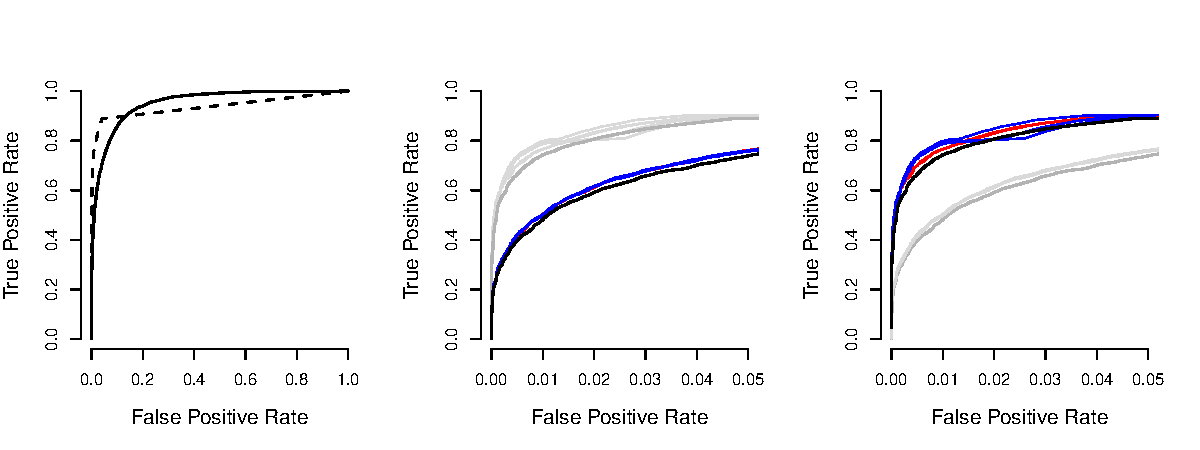
\includegraphics[width=7in]{Figures/roc.pdf}}
\caption{\label{roc} ROC curve as averaged across 60-sequence simulation set. A) Unfiltered alignments for FUBAR (dashed) and PAML (solid). Note that neither method achieved FPRs greater than shown. B) FUBAR in color with PAML results shown in grey. C) PAML in color with FUBAR results shown in grey.}
\end{figure*}



\begin{figure*}[H]
\centerline{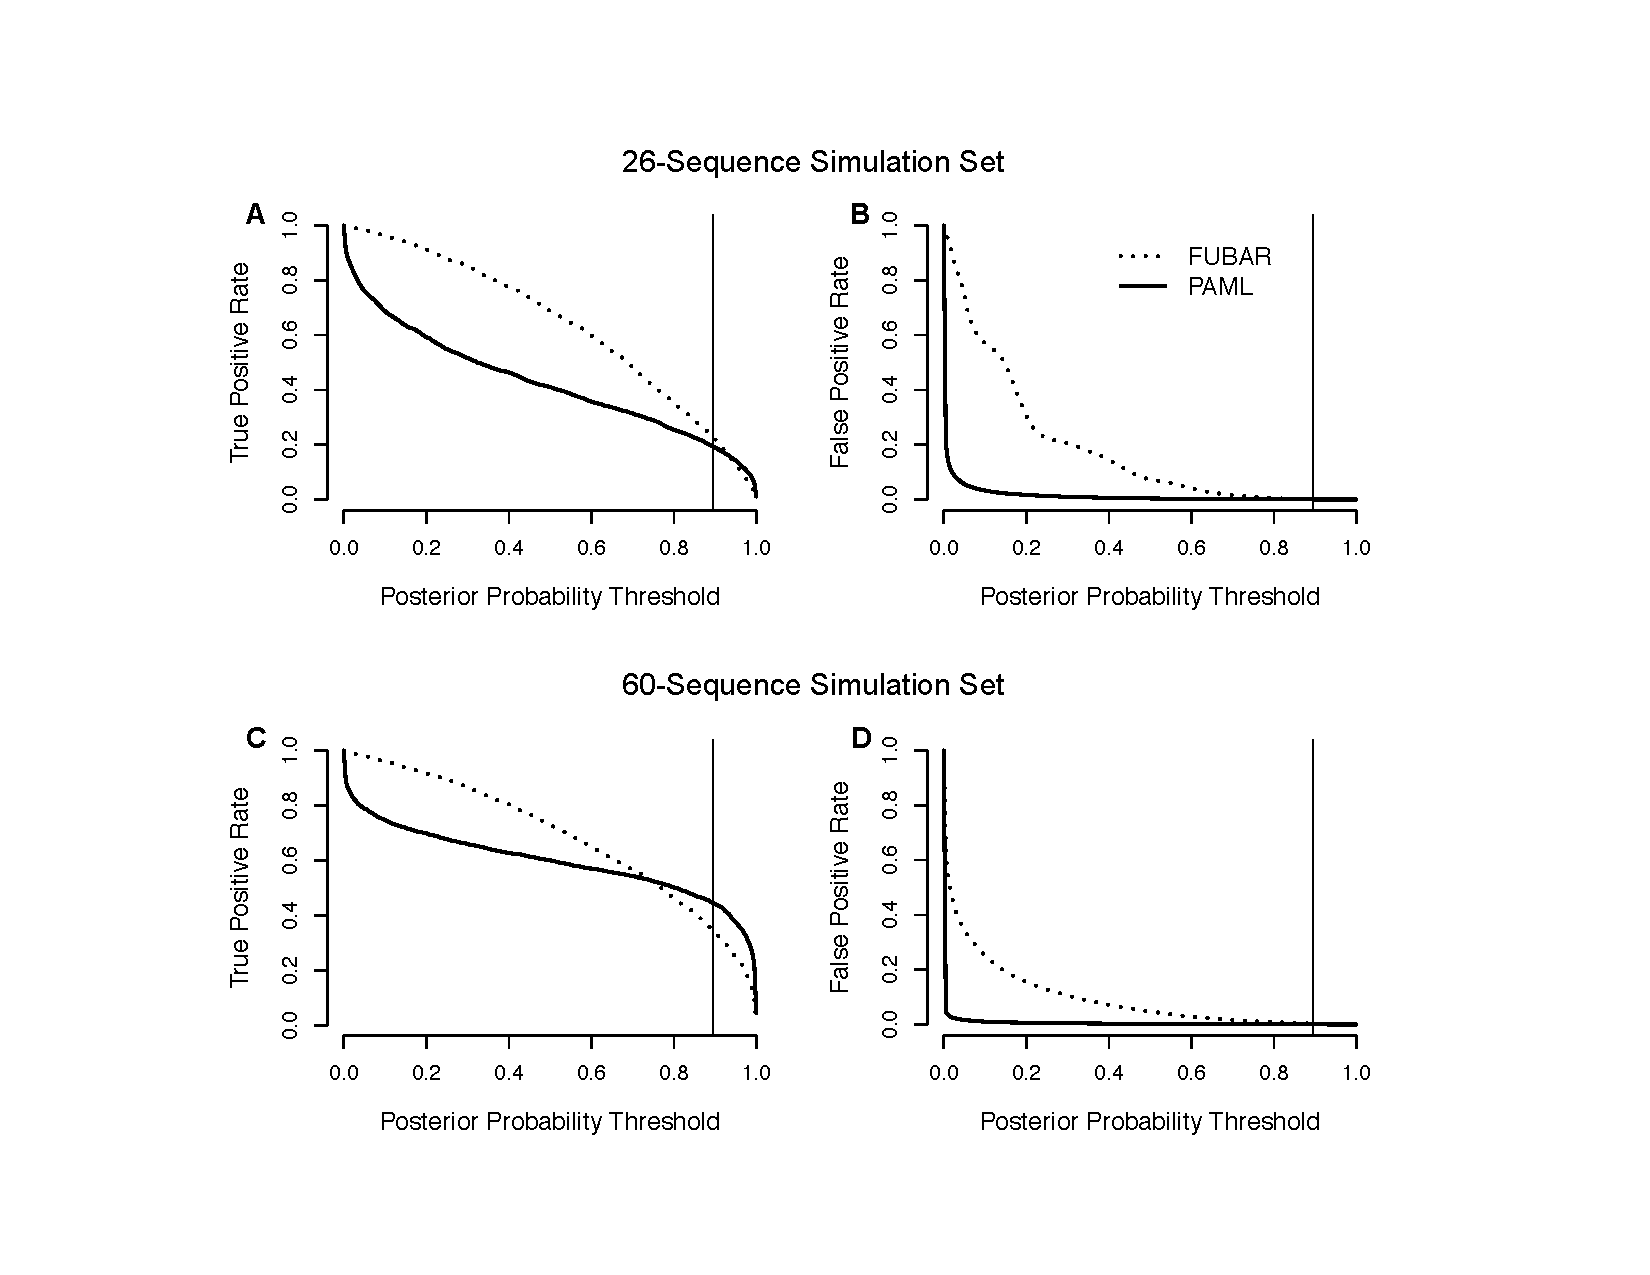
\includegraphics[width=7in]{Figures/tprfpr.pdf}}
\caption{\label{tprfpr} True and false positive rates recovered from FUBAR (dashed lines) and PAML (solid lines) analysis with unfiltered alignments, averaged across the 26-sequence and the 60-sequence simulation sets, against across posterior probability thresholds used to call sites as positively selected. Vertical lines indicate the posterior probability threshold of 0.9 used in the present study to call positively-selected sites. A) TPR, 26-sequence set. B) FPR, 26-sequence set. C) TPR, 60-sequence set. D) FPR, 60-sequence set.  As the number of sequences increased, PAML's TPR improved at lower posterior probabilities, while its FPR remained remarkably low across all posterior probabilities for both simulation sets. While FUBAR's performance did improve with the inclusion of more sequences, its overall TPR behavior did not change as dramatically as did PAML's.}
\end{figure*}



\begin{figure*}[H]
\centerline{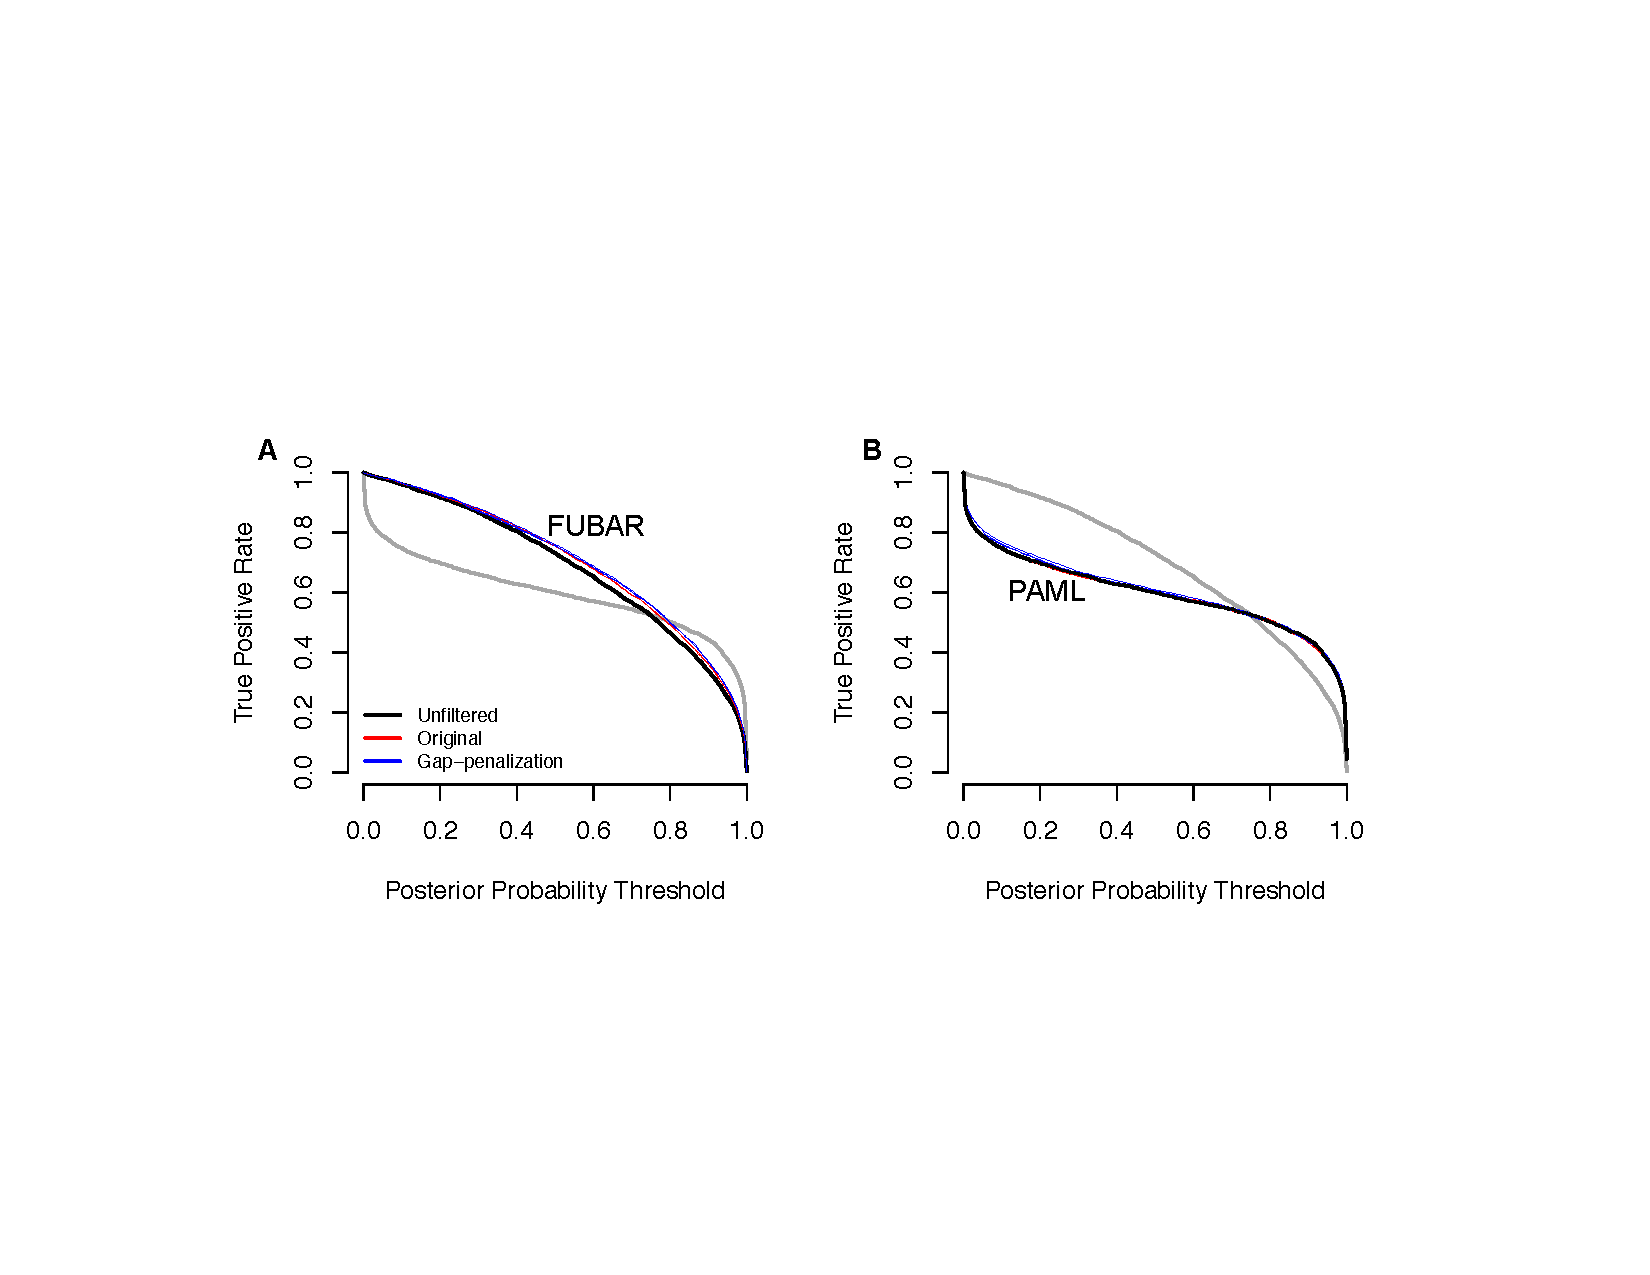
\includegraphics[width=7in]{Figures/fulltpr.pdf}}
\caption{\label{fulltpr} True positive rate against posterior probability threshold for calling positively selected sites, averaged across the 60-sequence simulation set. A) FUBAR in color with PAML results shown in grey. B) PAML in color with FUBAR results shown in grey. Filtered alignments behave similarly to unfiltered alignments across all posterior probabilities.}
\end{figure*}



\begin{table}[H]
\caption {\label{tab:penalmodel} Comparison between original and gap-penalization normalization schemes on TPR of positive-selection inference.}
\begin{tabular}{l l l l l l}
\hline\noalign{\smallskip}
\multicolumn{1}{c}{Simulation Set} & \multicolumn{1}{c}{Method} & \multicolumn{1}{c}{Guidance} & \multicolumn{1}{c}{BMweights} & \multicolumn{1}{c}{PDweights} \\
\noalign{\smallskip}\hline\noalign{\smallskip}
11 taxa  & FUBAR & 0.001 (0.98\%) & $-1.76\times10^{-5}$ (-0.002\%) & 0.001 (0.95\%)\\
              & PAML & $-2.68\times10^{-4}$ (-0.31\%) & $2.57\times10^{-5}$ (0.03\%) & -0.001 (-1.50\%)\\
\hline
26 taxa   & FUBAR & 0.0032 (1.38\%) & $4.02\times10^{-4}$ (1.75\%) & 0.0018 (0.77\%)\\
              & PAML & \textbf{0.006 (3.02\%)}$^{\ast}$ & \textbf{0.007 (3.32\%)}$^{\ast\ast}$ & \textbf{0.006 (2.89\%)}$^{\ast}$ \\
\hline
60 taxa  & FUBAR & \textbf{0.010 (2.67\%)}$^{\ast}$ & \textbf{0.012 (3.30\%)}$^{\ast\ast}$  & 0.005  (1.29\%)\\
              & PAML & -0.002 (-0.46\%) & 0.010 (2.23\%) & 0.008 (1.84\%) \\
\hline
158 taxa & FUBAR & 0.003 (0.79\%) & 0.002 (0.48\%) & 0.001 (0.28\%)\\
\hline
\end{tabular}
\newline
\textsc{note.}--- Significance levels: $^{\ast\ast} P < 0.01$; $^{\ast} P < 0.05$. Each column displays the magnitude of TPR difference between normalization schemes, represented as gap-penalization minus original, for each algorithm, respectively. Percentage changes from the original normalization scheme are shown in parentheses. All significance levels were corrected for multiple comparisons using the R multcomp package \citep{Hothorn2008}.
\end{table}


\begin{table}
\caption {\label{tab:casemodel} Effect of alignment filtering on TPR of positive-selection inference.}
\begin{tabular}{c c c l l l}
\hline\noalign{\smallskip}
& & & \multicolumn{3}{c}{Filtered TPR} \\
\cline{4-6}\noalign{\smallskip}
Simulation Set & Method & Unfiltered TPR & \multicolumn{1}{c}{GuidanceP} & \multicolumn{1}{c}{BMweightsP} & \multicolumn{1}{c}{PDweightsP} \\ 
\hline\noalign{\smallskip}
11 taxa  & FUBAR & 0.108 & 0.109  (1.04\%)   & 0.110  (1.86\%)  & 0.110  (1.37\%)        \\
              & PAML &  0.087 & 0.088  (0.49\%) &  0.088  (0.83\%)   & 0.088  (0.79\%)        \\
\hline
26 taxa   & FUBAR &  0.229 & 0.232 (1.54\%)  & 0.233 (1.83\%) & 0.233 (1.91\%)         \\
              & PAML & 0.194 & \textbf{0.204 (4.87\%)}$^{\ast}$ & \textbf{0.203 (4.56\%)}$^{\ast}$ & \textbf{0.203 (4.58\%)}$^{\ast}$   \\
\hline
60 taxa  & FUBAR & 0.345 & \textbf{0.379 (9.92\%)}$^{\ast\ast}$ & \textbf{0.377 (9.31\%)}$^{\ast\ast}$ & \textbf{0.375 (8.75\%)}$^{\ast\ast}$  \\
              & PAML & 0.447 & 0.447 (0.19\%) & 0.440 (-1.43\%) & 0.445 (-0.30\%) \\
\hline
158 taxa & FUBAR & 0.374 & \textbf{0.388 (3.89\%)}$^{\ast\ast}$ & \textbf{0.387 (3.68\%)}$^{\ast\ast}$ & \textbf{0.387 (3.47\%)}$^{\ast\ast}$  \\
\hline
\end{tabular}
\newline
\textsc{note.}--- Significance levels: $^{\ast\ast} P < 10\times10^{-5}$; $^{\ast} P < 10\times10^{-4}$. Unfiltered TPR: average TPR for unfiltered alignments; Filtered TPR: average TPR for alignments filtered with each respective algorithm, with percent change from unfiltered alignment shown in parentheses. All significance levels are relative to the given simulation set's unfiltered alignment. We detected no significant TPR differences among filters tested within sequence simulation sets. All significance levels were corrected for multiple comparisons using the R multcomp package \citep{Hothorn2008}.

\end{table}



\begin{table}
\caption {\label{tab:cutoffs} Effect of masking cutoff on TPR of positive-selection inference.}
\begin{tabular}{c c c c c}
\hline\noalign{\smallskip}
Simulation Set & Method & 0.5 TPR & 0.9 TPR & Percent TPR Decrease \\ 
\hline\noalign{\smallskip}
11 taxa & FUBAR & 0.109 & 0.104 & 4.99\%$^{\ast}$\\ 
             & PAML   & 0.087 & 0.080 & 8.36\%$^{\ast}$\\ 
26 taxa & FUBAR & 0.232 & 0.220 & 5.28\%$^{\ast\ast}$\\
             & PAML   & 0.204 & 0.195 &  4.34\%$^{\ast}$\\ 
60 taxa & FUBAR & 0.379 & 0.281 & 25.8\%$^{\ast\ast\ast}$\\
             & PAML    & 0.447 & 0.327 & 27.0\%$^{\ast}$\\ 
158 taxa & FUBAR & 0.388 & 0.374  & 3.57\%$^{\ast\ast\ast}$\\
\hline
\end{tabular}
\newline
\textsc{note.}--- Significance levels: $^{\ast\ast\ast} P < 1\times10^{-6}$; $^{\ast\ast} P < 1\times10^{-5}$; $^{\ast} P < 1\times10^{-3}$. 
0.5 TPR: average TPR for alignments masked at a cutoff of 0.5 with GuidanceP; 0.9 TPR: average TPR for alignments masked at a cutoff of 0.9 with GuidanceP; Percent TPR Decrease: average percent decrease in TPR recovered between alignments masked at cutoffs of 0.5 and 0.9. All significance levels were corrected for multiple comparisons using the R multcomp package \citep{Hothorn2008}.
\end{table}


\bibliographystyle{MBE}
\bibliography{citations}	

\end{document}